% !TEX program = xelatex
\documentclass[11pt]{article}
\usepackage{fullpage}  
\usepackage{graphicx}
\usepackage{amssymb}
\usepackage{amsmath}
\usepackage{bm}
\usepackage{fancyvrb}
% \usepackage[utf8]{ctex}
\usepackage{xeCJK}
\usepackage{listings} 
\usepackage{xcolor}
\usepackage{titlesec}
\usepackage{enumerate}
\usepackage{enumitem}
\usepackage{booktabs}
\usepackage{bookmark}
\usepackage{multirow}
\usepackage{bbm}
% \usepackage[colorlinks=true,linkcolor=cyan]{hyperref}
\usepackage{geometry}
\geometry{a4paper,left=1.5cm,right=1.5cm,top=2cm,bottom=2cm}
\setlist[enumerate,1]{label=\alph*.,itemsep=-5pt}
\renewcommand{\baselinestretch}{1.2} % 行间距
\usepackage{fontspec}
\setcounter{tocdepth}{1} % 目录显示深度
\usepackage{caption}
\usepackage{subcaption}
\lstset{ 
    keywordstyle= \color{ blue!80!black!80!},
    commentstyle= \color{red!80!green!80!}, 
	backgroundcolor=\color{black!5!},
	basicstyle=\tiny \monaco
	%escapeingside={\%*}{*)}
    frame=shadowbox, % 阴影效果
    rulesepcolor= \color{ red!20!green!20!blue!20} ,
    %xleftmargin=2em,xrightmargin=2em, aboveskip=1em,
    %framexleftmargin=2em
	numberstyle=\tiny,
	basicstyle=\ttfamily,
}
% \begin{lstlisting}[language=R] 
% \end{lstlisting}

\title{\vspace{-2em}\textbf{StatComp HW2}}
\author{Jiang Wenxin 16342067}
\date{\today}
\begin{document}
\maketitle
\tableofcontents
\section{Metropolis-Hastings Algorithm}
\textbf{7.1} The goal of this problem is to investigate the role of the proposal distribution in a Metropolis-Hastings algorithm designed to simulate from the posterior distribution of a parameter $\delta .$ In part (a), you are asked to simulate data from a distribution with $\delta$ known. For parts (b)-(d), assume $\delta$ is unknown with a Unif(0,1) prior distribution for $\delta$. For parts (b)-(d), provide an appropriate plot and a table summarizing the output of the algorithm. To facilitate comparisons, use the same number of iterations, random seed, starting values, and burn-in period for all implementations of the algorithm.
\begin{enumerate}
    \item Simulate 200 realizations from the mixture distribution in Equation (7.6) with $\delta=0.7.$ Draw a histogram of these data.
    \item Implement an independence chain MCMC procedure to simulate from the posterior distribution of $\delta$, using your data from part (a).\\ 
    Given $\mathbf{X}^{(t)}=\mathbf{x}^{(t)},$ the algorithm generates $\mathbf{X}^{(t+1)}$ as follows:
    \begin{enumerate}
        \item Sample a candidate value $\mathbf{X}^{*}$ from a proposal distribution $g\left(\cdot \mid \mathbf{x}^{(t)}\right)$.
        \item Compute the Metropolis-Hastings ratio $R\left(\mathbf{x}^{(t)}, \mathbf{X}^{*}\right),$ where
    \begin{align*}
        R(\mathbf{x}^{(t)}, \mathbf{X}^{*})=\frac{f(\mathbf{X}^{*}) g(\mathbf{x}^{(t)} \mid \mathbf{X}^{*})}{f(\mathbf{x}^{(t)}) g(\mathbf{X}^{*} \mid \mathbf{x}^{(t)})}
    \end{align*}
        \item Sample a value for $\mathbf{X}^{(t+1)}$ according to the following:
        \begin{align*}
            \mathbf{X}^{(t+1)}=\left\{\begin{array}{ll}
            \mathbf{X}^{*} & \text { with probability } \min \left\{R\left(\mathbf{x}^{(t)}, \mathbf{X}^{*}\right), 1\right\} \\
            \mathbf{x}^{(t)} & \text { otherwise. }
            \end{array}\right.
        \end{align*}
        \item Increment $t$ and return to step 1.
    \end{enumerate}
    \item Implement a random walk chain with $\delta^{*}=\delta^{(t)}+\epsilon$ with $\epsilon \sim \operatorname{Unif}(-1,1).$
    \item Reparameterize the problem letting $U=\log \{\delta /(1-\delta)\}$ and $U^{*}=u^{(t)}+\epsilon .$ Implement a random walk chain in $U$-space as in Equation (7.8).
    \item Compare the estimates and convergence behavior of the three algorithms.
\end{enumerate}
\textbf{Ans.}
\begin{enumerate}
    \item R code available at Section~\ref{sec:mhgen}. The histogram of these data shows in Figure~\ref{fig:hist}.
        \begin{figure}[!htb]
            \begin{center}
                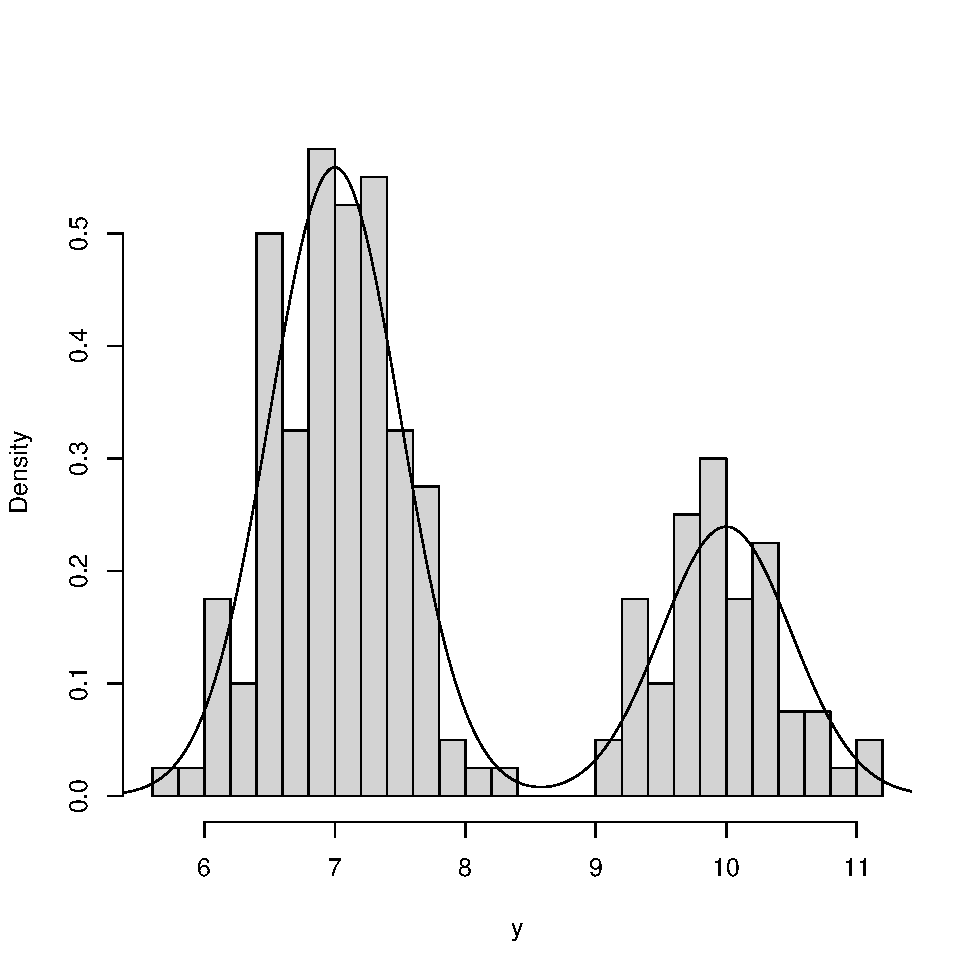
\includegraphics[width=0.6\linewidth]{img/mhgen-1.pdf}
            \end{center}
            \caption{Histogram of Data and Plot of Mixture Distribution}
            \label{fig:hist}
        \end{figure}
    \item In an independence chain, the proposal distribution $g\left(\mathbf{x}^{*} \mid \mathbf{x}^{(t)}\right)=g\left(\mathbf{x}^{*}\right)$ and the Metropolis-Hastings ratio is$$R\left(\mathbf{x}^{(t)}, \mathbf{X}^{*}\right)=\frac{f\left(\mathbf{X}^{*}\right) g\left(\mathbf{x}^{(t)}\right)}{f\left(\mathbf{x}^{(t)}\right) g\left(\mathbf{X}^{*}\right)}.$$Use the prior distribution Unif(0,1) as a proposal distribution in an independence chain. Thus, $$R\left(\boldsymbol{\theta}^{(t)}, \boldsymbol{\theta}^{*}\right)=\frac{L\left(\boldsymbol{\theta}^{*} \mid \mathbf{y}\right)}{L\left(\boldsymbol{\theta}^{(t)} \mid \mathbf{y}\right)}.$$ R code available at Section~\ref{sec:mhic}. The sample path and the histogram of independence chain show in Figure~\ref{fig:mhic}.
    \begin{figure}[!hbt]
        \begin{center}
            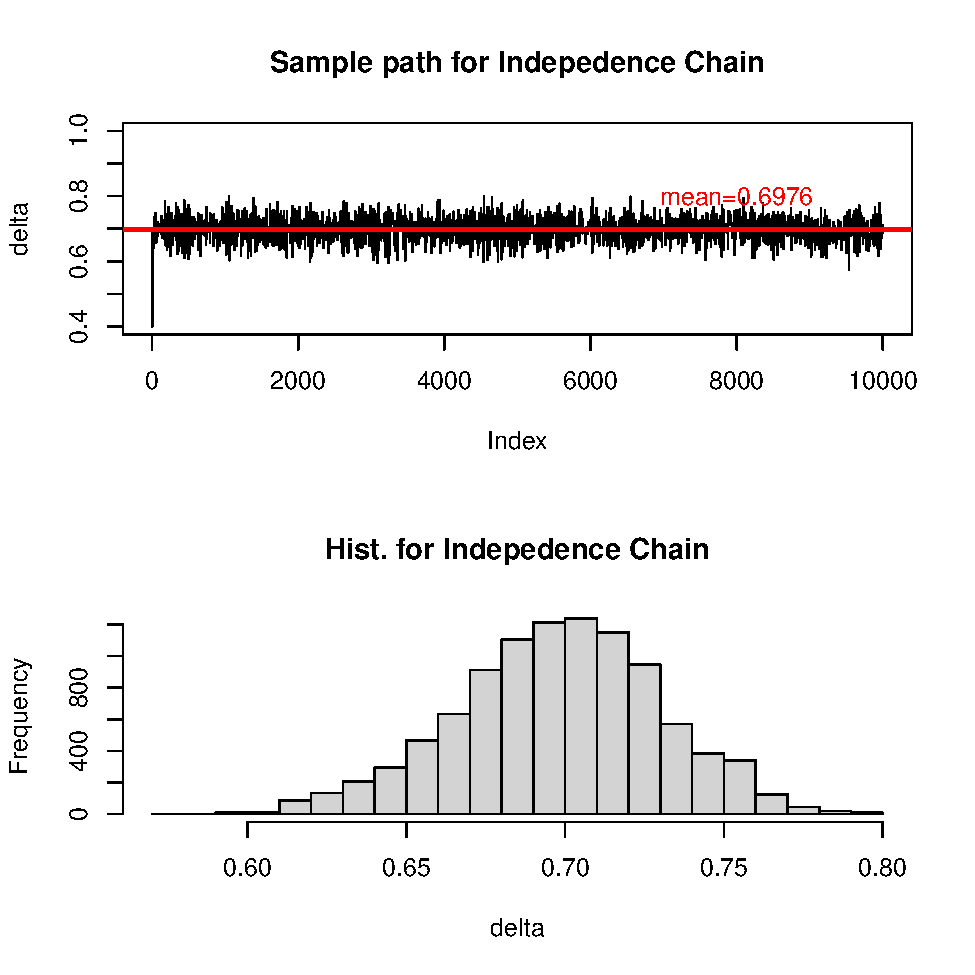
\includegraphics[width=0.6\textwidth]{img/mhic-1.pdf}
        \end{center}
        \caption{Sample Path and the Histogram of Independence Chain Starting at $\delta=0.4$}
        \label{fig:mhic}
    \end{figure}
    \item In a random walk chain $\mathbf{X}^{*}$ is generated by drawing $\boldsymbol{\epsilon} \sim h(\boldsymbol{\epsilon})$  and $\mathbf{X}^{*}=\mathbf{x}^{(t)}+\boldsymbol{\epsilon}.$ Thus, $g\left(\mathbf{x}^{*} \mid \mathbf{x}^{(t)}\right)=h\left(\mathbf{x}^{*}-\mathbf{x}^{(t)}\right) .$ Since proposal density $g$ is symmetric about zero. $g\left(\mathbf{x}^{*} \mid \mathbf{x}^{(t)}\right)=g\left(\mathbf{x}^{(t)} \mid \mathbf{x}^{*}\right)$. Therefore, the Metropolis-Hastings ratio in this case is $$R(\delta^{(t)},\delta^{*})=\frac{f\left(\delta^{*}\right)}{f\left(\delta^{(t)}\right) }.$$Let $U=\operatorname{logit}\{\delta\}=\log \{\delta /(1-\delta)\}$. R code available at Section~\ref{sec:mhrw}. The sample path of random walk chain in $\delta$- space shows in Figure~\ref{fig:mhrw}.
    \item the Metropolis-Hastings ratio in this case is $$R(\delta^{(t)},\delta^{*})=\frac{f\left(\operatorname{logit}^{-1}\left\{u^{*}\right\}\right)\left|J\left(u^{*}\right)\right|}{f\left(\operatorname{logit}^{-1}\left\{u^{(t)}\right\}\right)\left|J\left(u^{(t)}\right)\right|},$$where $\delta=\operatorname{logit}^{-1}\{U\}=\exp \{U\} /(1+\exp \{U\})$. R code available at Section~\ref{sec:mhrw}. The sample path of random walk chain in U-space shows in Figure~\ref{fig:mhrw}.
    \begin{figure}[htbp]
        \begin{center}
            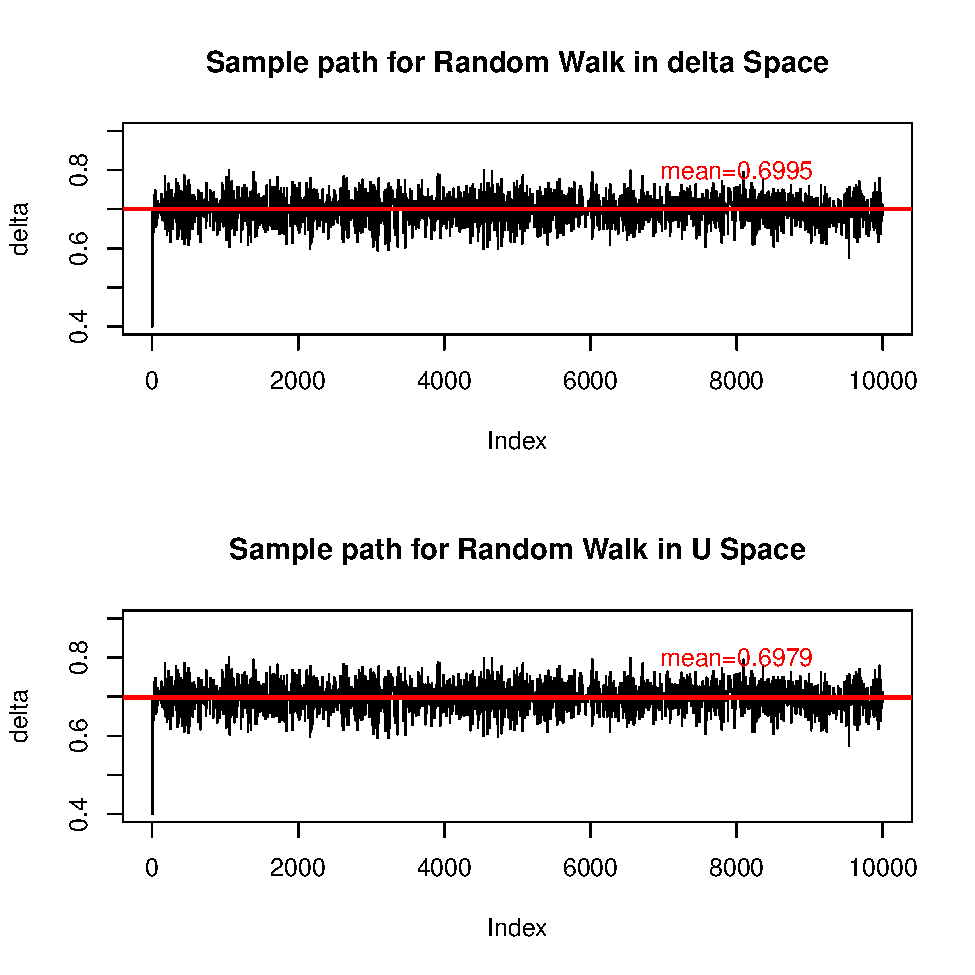
\includegraphics[width=0.6\textwidth]{img/mhrw-1.pdf}
        \end{center}
        \caption{Sample Path of Random Walk in delta Space and U Space Starting at $\delta=0.4$}\label{fig:mhrw}
    \end{figure}  
    \item  The sample path plots above show that all three Metropolis-Hastings algorithms move quickly away from its starting value and seems easily able to sample values from all portions of the parameter space supported by the posterior for $\delta$, which is good mixing. From Table \ref{tab:mh}, we can obtain that three algorithms converge and do not sensitive to the starting points. This illustrates that proposal distributions we chose could generate reliable estimation of $\delta$.
    \begin{table}[htbp]
        \centering
        \caption{Estimations by Different MH Algorithms with Different Starting Points}\label{tab:mh}
        \begin{tabular}{lcccc} 
        \toprule
        Initial Value              & 0.2    & 0.4    & 0.6    & 0.8     \\ 
        \midrule
        Indepedence Chain          & 0.6977 & 0.6976 & 0.6986 & 0.6988  \\
        Random Walk in delta Space & 0.7001 & 0.6995 & 0.6992 & 0.6989  \\
        Random Walk in U Space     & 0.6982 & 0.6979 & 0.6979 & 0.6989  \\
        \bottomrule
        \end{tabular}
    \end{table}
\end{enumerate}


\section{Gibbs Sampler: Poisson Process with Change Point}
\textbf{7.6} Problem 6.4 introduces data on coal-mining disasters from 1851 to 1962. For these data, assume the model $$
x_{j} \sim\left\{\begin{array}{ll}
\operatorname{Poi}\left(\lambda_{1}\right), & j=1, \ldots, \theta \\
\text {Poi}\left(\lambda_{2}\right), & j=\theta+1, \ldots , 112
\end{array}\right.
$$
Assume $\lambda_{i} \mid \alpha \sim \operatorname{Gamma}(3, \alpha)$ for $i=1,2,$ where $\alpha \sim \operatorname{Gamma}(10,10),$ and assume $\theta$ follows a discrete uniform distribution over $\{1, \ldots, 111\} .$ The goal of this problem is to estimate the posterior distribution of the model parameters via a Gibbs sampler.
\begin{enumerate}
    \item Derive the conditional distributions necessary to carry out Gibbs sampling for the change-point model.
    \item Implement the Gibbs sampler. Use a suite of convergence diagnostics to evaluate the convergence and mixing of your sampler.
    \item Construct density histograms and a table of summary statistics for the approximate posterior distributions of $\theta, \lambda_{1},$ and $\lambda_{2} .$ Are symmetric highest posterior density (HPD) intervals appropriate for all of these parameters?
    \item Interpret the results in the context of the problem.
\end{enumerate}
\textbf{Ans.}
\begin{enumerate}
    \item Let the set of unknown parameter be $\mathbf{\phi}=(\lambda_1,\lambda_2,\theta,\alpha)$. For convenience, donate $n=112$ as the number of year and
    \begin{align*}
        \lambda_1 &\sim \Gamma(a_1,\alpha),\\
        \lambda_2 &\sim \Gamma(a_2,\alpha),\\
        \alpha &\sim \Gamma(b,b),\\
        \theta&\sim \operatorname{Unif}(1,n-1).
    \end{align*}
    \par Then the posterior is
    \begin{align*}
        &\pi(\mathbf{\phi} \mid \mathbf{x})\\
        \propto& L( \mathbf{x}\mid \mathbf{\phi}) p(\lambda_1\mid\alpha) p(\lambda_2\mid\alpha) p(\alpha) p(\theta)\\
        =&\left[\prod_{i=1}^{\theta} \frac{e^{-\lambda_1} \lambda_1^{x_{i}}}{x_{i} !}\right] \left[\prod_{i=\theta+1}^{n} \frac{e^{-\lambda_2} \lambda_2^{x_{i}}}{x_{i} !}\right]
        \left[\frac{\alpha^{a_1}}{\Gamma(a_1)} \lambda_1^{a_1-1} e^{-\alpha \lambda_1}\right]
        \left[\frac{\alpha^{a_2}}{\Gamma(a_2)} \lambda_2^{a_2-1} e^{-\alpha \lambda_2}\right]
        \left[\frac{b^{b}}{\Gamma(b)} \alpha^{b-1} e^{-b \alpha}\right]
        \frac{1}{n-2}\\
        \propto&\left[ e^{-(\theta+\alpha)\lambda_1} \lambda_1^{\sum\limits_{i=1}^{\theta} x_i+a_1-1} \right]
        \left[ e^{-(n-\theta+\alpha)\lambda_2} \lambda_2^{\sum\limits_{i=\theta+1}^{n} x_i+a_2-1} \right] \left[ e^{-b\alpha} \alpha^{a_1+a_2+b-1} \right]\\ 
        \propto& \left[ e^{-(b+\lambda_1+\lambda_2)\alpha} \alpha^{a_1+a_2+b-1} \right] f(\theta,\lambda_1,\lambda_2\mid \alpha,\mathbf{x})\\ 
        \propto& \exp\{\theta(\lambda_2-\lambda_1)\}\left( \frac{\lambda_2}{\lambda_1}\right)^{\sum\limits_{i=1}^{\theta} x_i} f(\alpha,\lambda_1,\lambda_2\mid \theta,\mathbf{x}).
    \end{align*}
    \par Thus, a Gibbs sampler can be constructed by simulating from the following conditional posterior distributions. 
    \begin{align*}
        \lambda_1 \mid \cdot &\sim \Gamma(a_1+\sum\limits_{i=1}^{\theta}x_i, \theta+\alpha),\\
        \lambda_2 \mid \cdot &\sim \Gamma(a_2+\sum\limits_{i=\theta+1}^{n}x_i,n- \theta+\alpha),\\
        \alpha  \mid \cdot&\sim \Gamma(a_1+a_2+b,b+\lambda_1+\lambda_2),\\
        \theta \mid \cdot&\sim  c\cdot \exp\{(\lambda_2-\lambda_1)\theta\}\left( \frac{\lambda_1}{\lambda_2} \right)^{\sum\limits_{i=1}^{\theta}x_i},
    \end{align*}
    where $c$ is a normalization parameter. Then, in this case, MCMC sampling from
    \begin{align*}
        \lambda_1 \mid \cdot &\sim \Gamma(3+\sum\limits_{i=1}^{\theta}x_i, \theta+\alpha),\\
        \lambda_2 \mid \cdot &\sim \Gamma(3+\sum\limits_{i=\theta+1}^{112}x_i,112- \theta+\alpha),\\
        \alpha  \mid \cdot&\sim \Gamma(16,10+\lambda_1+\lambda_2),\\
        \theta \mid \cdot &\sim c\cdot \exp\{(\lambda_2-\lambda_1)\theta\}\left( \frac{\lambda_1}{\lambda_2} \right)^{\sum\limits_{i=1}^{\theta}x_i}.
    \end{align*}
    \item R code at Section~\ref{sec:gs}
    \begin{itemize}
        \item \textbf{Sample Path Plots: }Figure~\ref{fig:gssp} shows that the chains are mixing well, quickly moves away from its starting value and the sample path will wiggle about vigorously in the region supported by $f$.
        \begin{figure}[!htbp]
            \begin{subfigure}[t]{0.49\textwidth}
                \centering
        %		 include first image
                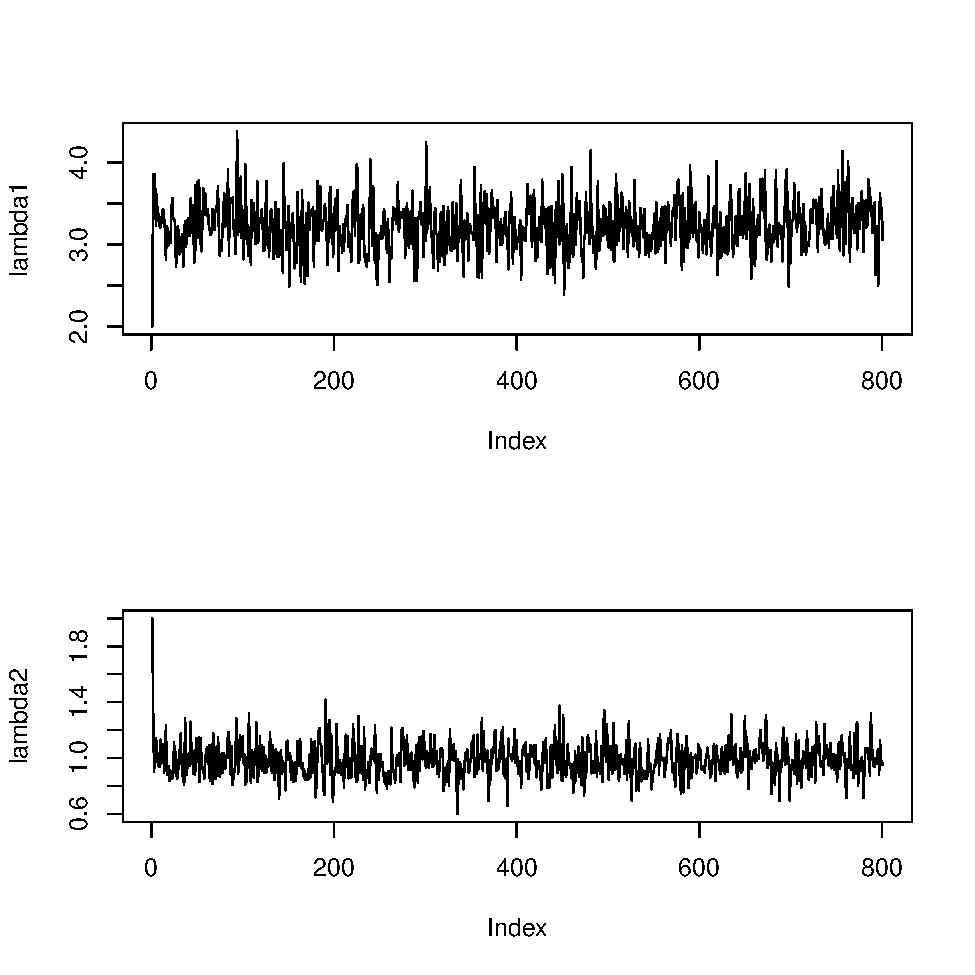
\includegraphics[width=\linewidth]{img/gssp-1.pdf}
                %\caption{}
            \end{subfigure}
            \begin{subfigure}[t]{0.49\textwidth}
                \centering
        %		 include second image
                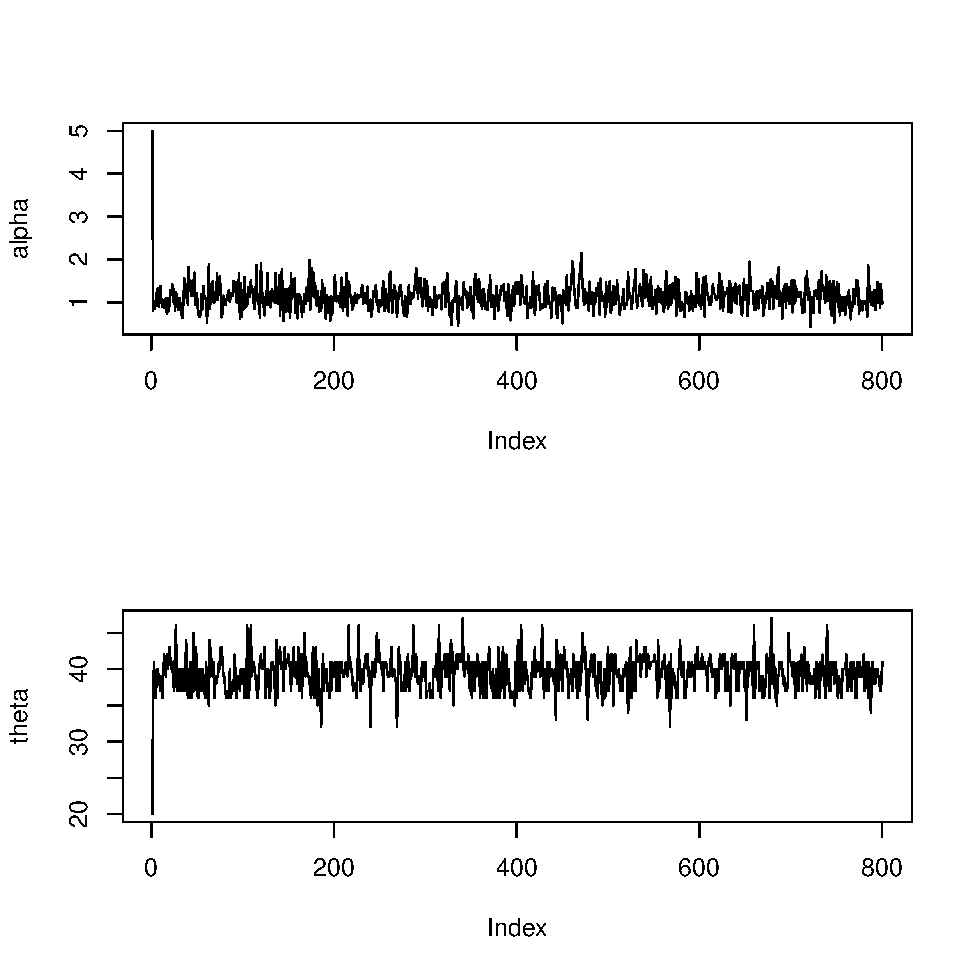
\includegraphics[width=\linewidth]{img/gssp-2.pdf}
                %\caption{}
            \end{subfigure}
            \caption{Sample Path Plots of change-points model with Gibbs sampler}
            \label{fig:gssp}
        \end{figure}
        \item \textbf{Cumulative Sum Diagnostic:} Let $h(x)=x$ and set burn-in period equals to 200. Computed using only the iterations of the chain that remain after removing burn-in values, we obtain the cumulative sum of each parameter in $\mathbf{\phi}$. The cumsum plots in Figure~\ref{fig:gscs} are very wiggly and have smaller excursions from 0 which indicate the chains are mixing well.
        \begin{figure}[!htbp]
            \begin{subfigure}[t]{0.49\textwidth}
                \centering
        %		 include first image
                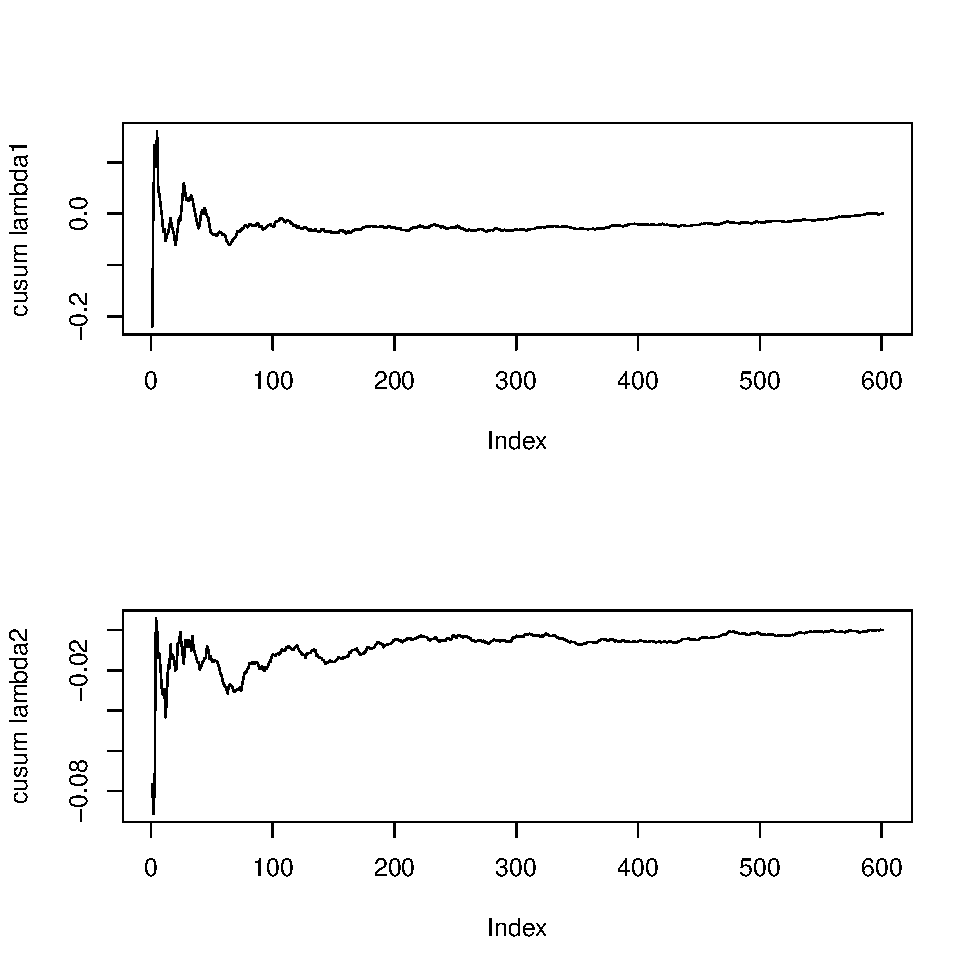
\includegraphics[width=\linewidth]{img/gscs-1.pdf}
                %\caption{}
            \end{subfigure}
            \begin{subfigure}[t]{0.49\textwidth}
                \centering
        %		 include second image
                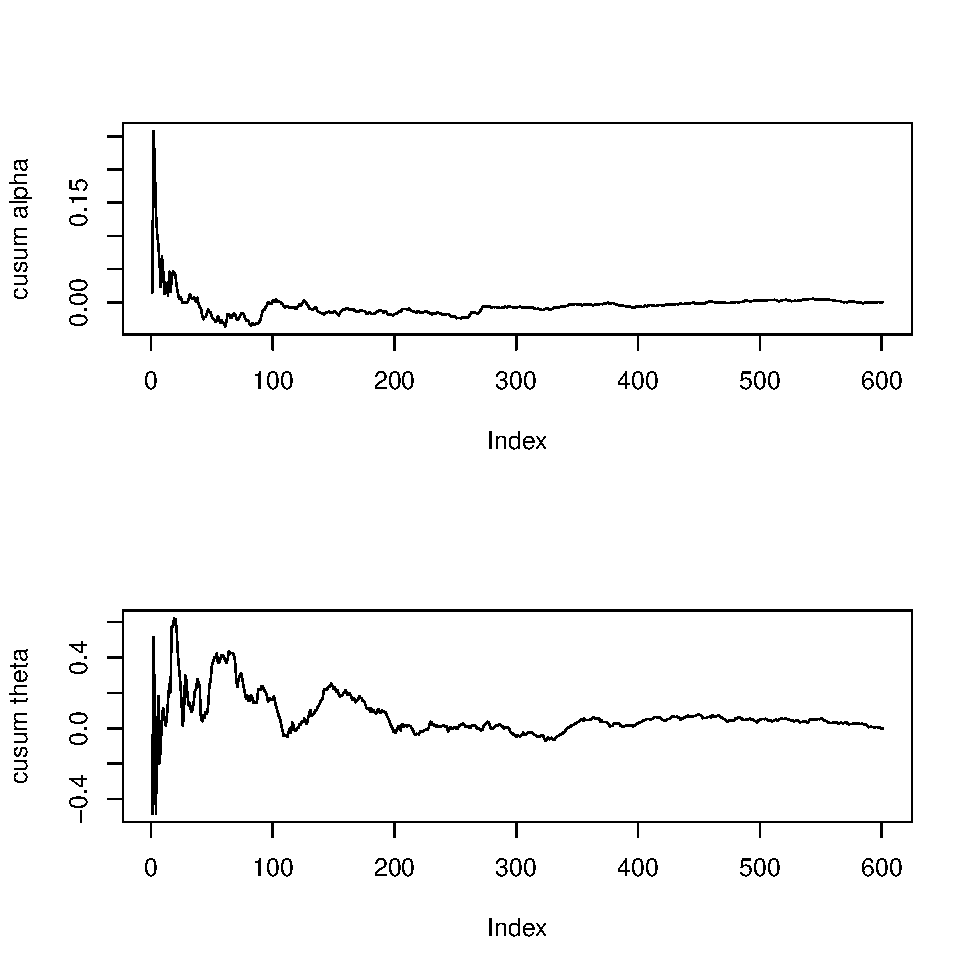
\includegraphics[width=\linewidth]{img/gscs-2.pdf}
                %\caption{}
            \end{subfigure}
            \caption{Cumulative Sum Plots of change-points model with Gibbs sampler}
            \label{fig:gscs}
        \end{figure}
        
        \item \textbf{Correlation Plot:} Figure~\ref{fig:gsac} and Figure~\ref{fig:gscc} show the correlation in the sequence of each parameter and cross parameters at different iteration lags. Cross-correlations are relative low and self-correlations vigorously wiggle about 0. This results indicates that the chains are performing well.
        \begin{figure}[!htb]
            \centering
            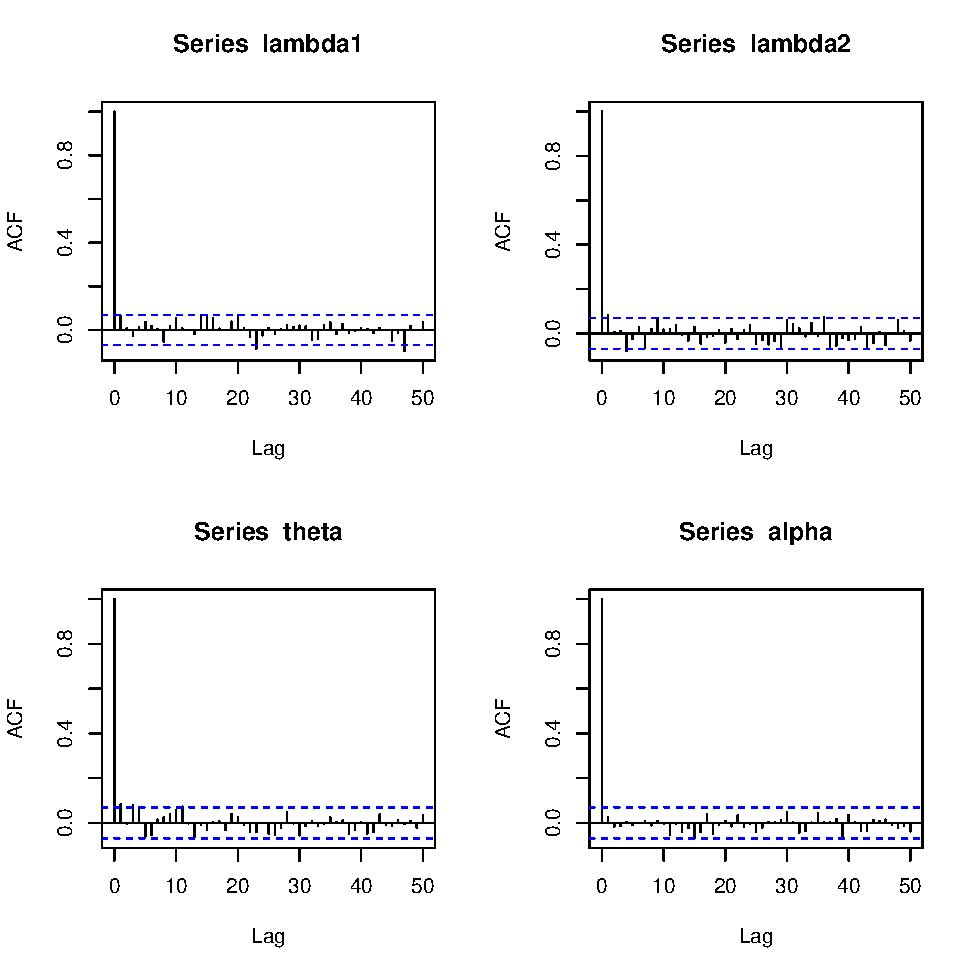
\includegraphics[width=0.7\linewidth]{img/gsac-1.pdf}
            \caption{Auto-correlation Plots of change-points model with Gibbs sampler.}
            \label{fig:gsac}
        \end{figure}
        \begin{figure}[!htb]
            \centering
            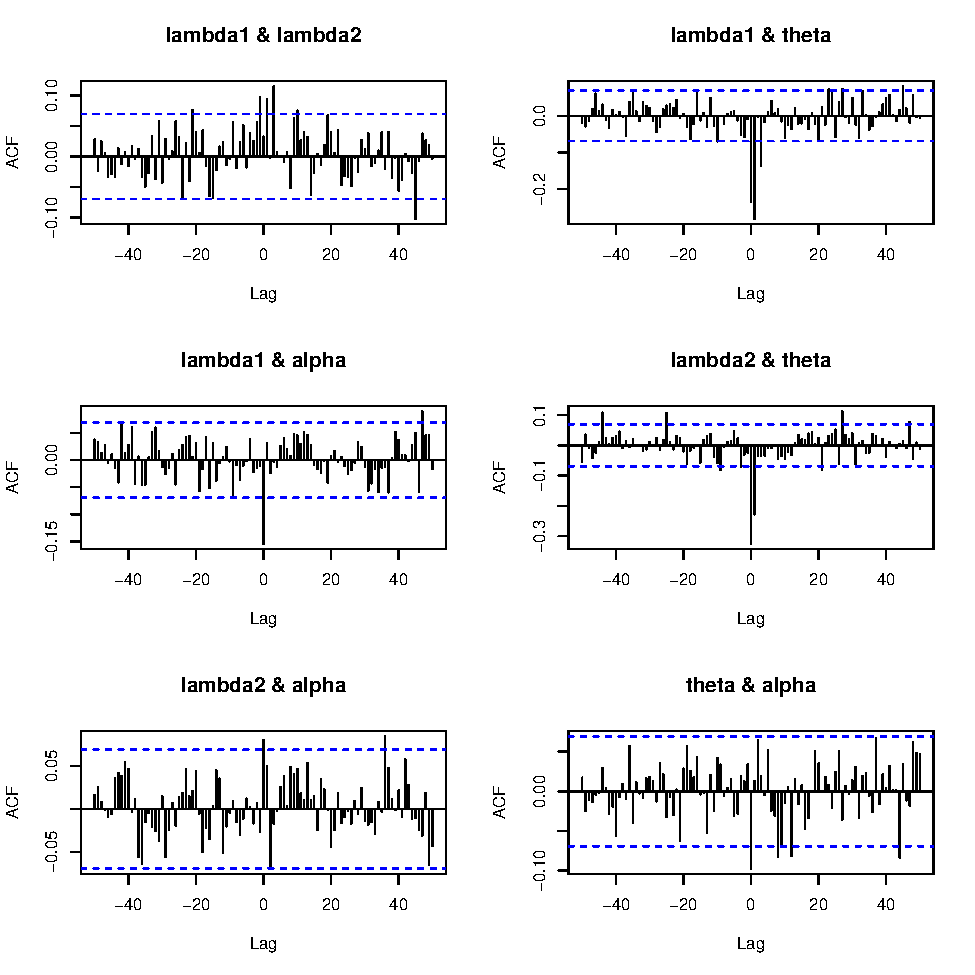
\includegraphics[width=0.8\linewidth]{img/gsac-2.pdf}
            \caption{Cross-correlation Plots of change-points model with Gibbs sampler.}
            \label{fig:gscc}
        \end{figure}
    \end{itemize}
    
    \item Figure~\ref{fig:gshist} construct the density histograms of the four parameters and Table~\ref{tab:gsss} summarizes them. Since the distribution of $\lambda_1$ and $\lambda_2$ are  unimodal and symmetric, a symmetric HPD is suitable for them. And since the distribution of $\theta$ is multimodal and $\alpha$ are not symmetric, a symmetric HPD is not suitable for them.
    \begin{figure}[!htb]
        \begin{subfigure}[t]{0.49\textwidth}
            \centering
    %		 include first image
            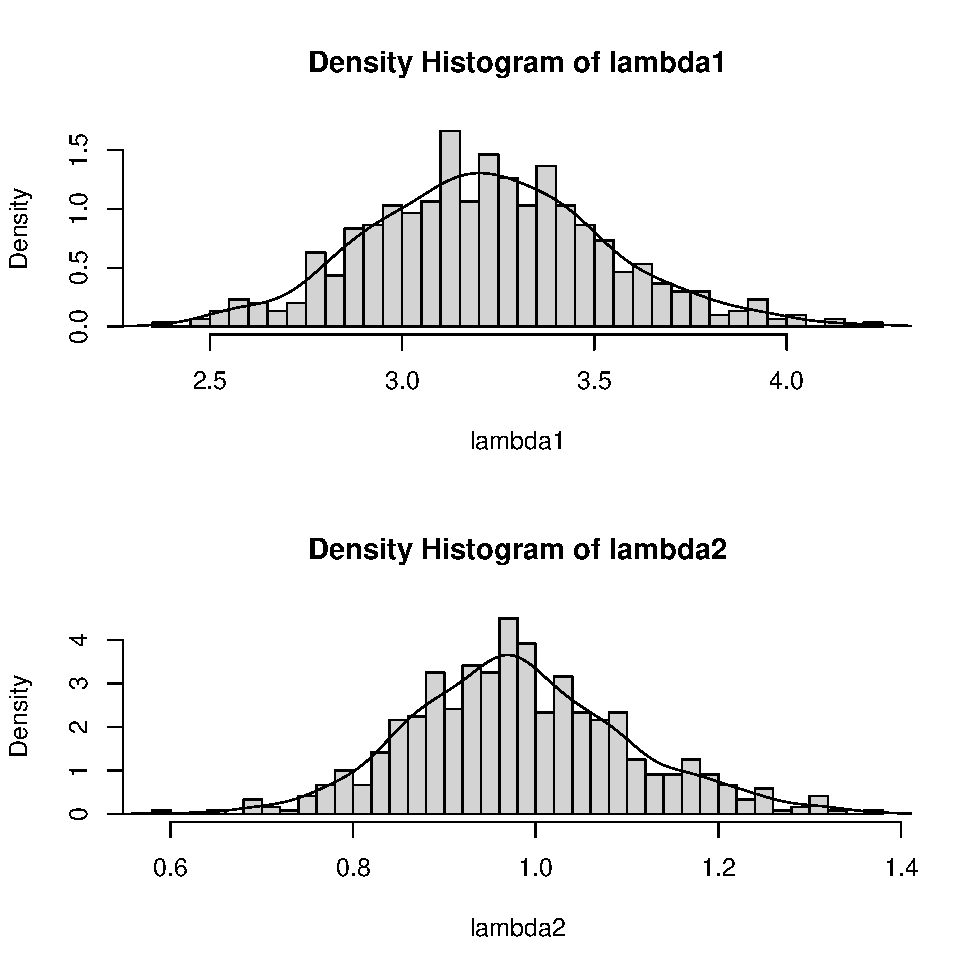
\includegraphics[width=\linewidth]{img/gshist-1.pdf}
            %\caption{}
        \end{subfigure}
        \begin{subfigure}[t]{0.49\textwidth}
            \centering
    %		 include second image
            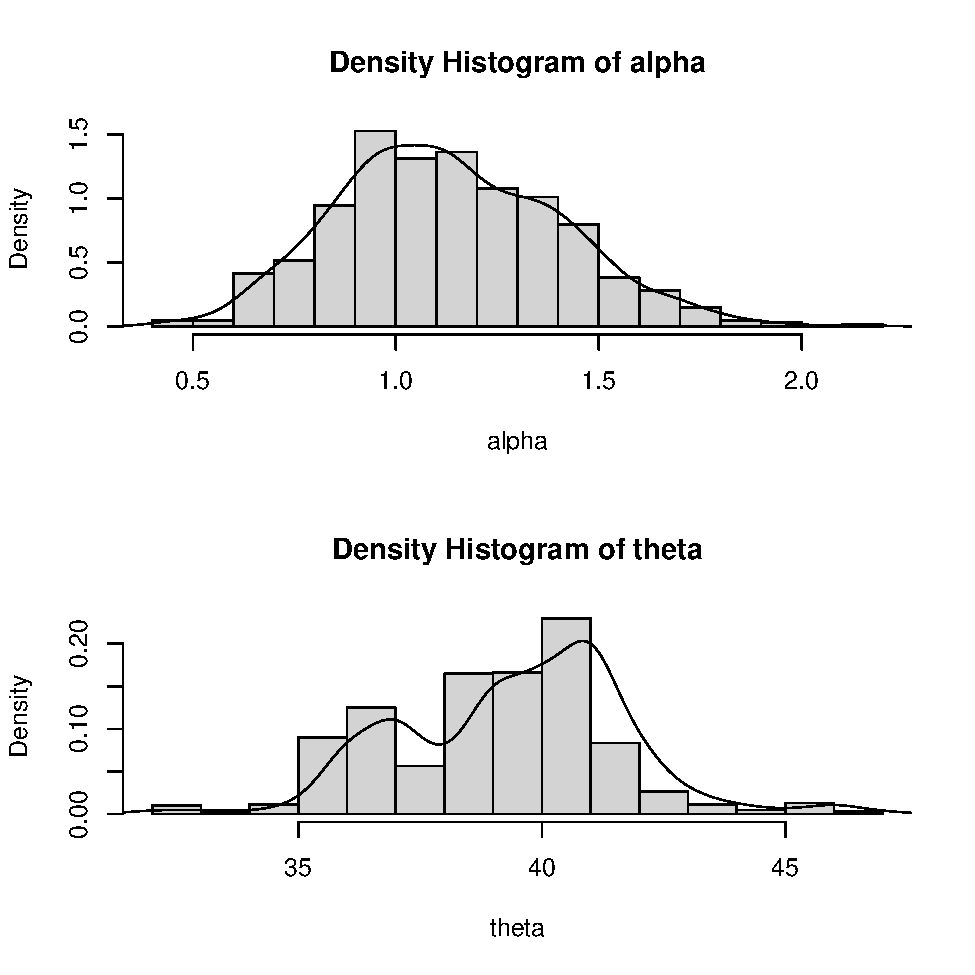
\includegraphics[width=\linewidth]{img/gshist-2.pdf}
            %\caption{}
        \end{subfigure}
        \caption{Density histograms of change-points model with Gibbs sampler}
        \label{fig:gshist}
    \end{figure}
    \begin{table}
        \centering
        \caption{Summary Statistics}
        \label{tab:gsss}
        \begin{tabular}{ccccccc} 
        \toprule
                & Min.   & 1st Qu. & Median & Mean   & 3rd Qu. & Max.   \\
        \midrule
        $\lambda_1$ & 2.386      & 3.009   & 3.220  & 3.223  & 3.425   & 4.249  \\
        $\lambda_2$ & 0.5974 & 0.8999   & 0.9751 & 0.9829 & 1.0543  & 1.3799      \\
        $\alpha$ &  0.4302 & 0.9376 & 1.1137 & 1.1310 & 1.3237 & 2.1526       \\
        $\theta$   & 32     & 38      & 40     & 39.49   & 41      & 47     \\
        \bottomrule
        \end{tabular}
        \end{table}
    \item The discussions above illustrate that chains in Gibbs sampling mixing well. 
\end{enumerate}

\section{Gibbs Sampler: Hierarchical Nested Model}
\textbf{7.7 }Consider a hierarchical nested model
$$
Y_{i j k}=\mu+\alpha_{i}+\beta_{j(i)}+\epsilon_{i j k},
$$
where $i=1, \ldots, I, j=1, \ldots, J_{i},$ and $k=1, \ldots, K .$ After averaging over $k$ for each $i$ and $j,$ we can rewrite the model (7.29) as
$$
Y_{i j}=\mu+\alpha_{i}+\beta_{j(i)}+\epsilon_{i j}, \quad i=1, \ldots, I, \quad j=1, \ldots, J_{i},
$$
where $Y_{i j}=\sum_{k=1}^{K} Y_{i j k} / K .$ Assume that $\alpha_{i} \sim N\left(0, \sigma_{\alpha}^{2}\right), \beta_{j(i)} \sim N\left(0, \sigma_{\beta}^{2}\right),$ and $\epsilon_{i j} \sim$
$N\left(0, \sigma_{\epsilon}^{2}\right),$ where each set of parameters is independent a priori. Assume that $\sigma_{\alpha}^{2}, \sigma_{\beta}^{2},$ and $\sigma_{\epsilon}^{2}$ are known. To carry out Bayesian inference for this model, assume an improper flat prior for $\mu,$ so $f(\mu) \propto 1 .$ We consider two forms of the Gibbs sampler for this problem.
\begin{enumerate}
    \item Let $n=\sum_{i} J_{i}, y_{. .}=\sum_{i j} y_{i j} / n,$ and $y_{i .}=\sum_{j} y_{i j} / J_{i}$ hereafter. Show that at iteration $t,$ the conditional distributions necessary to carry out Gibbs sampling for this model are given by
    $$
    \begin{aligned}
    \mu^{(t+1)} \mid\left(\boldsymbol{\alpha}^{(t)}, \boldsymbol{\beta}^{(t)}, \mathbf{y}\right) & \sim N\left(y_{..}-\frac{1}{n} \sum_{i} J_{i} \alpha_{i}^{(t)}-\frac{1}{n} \sum_{j(i)} \beta_{j(i)}^{(t)}, \frac{\sigma_{\epsilon}^{2}}{n}\right), \\
    \alpha_{i}^{(t+1)} \mid\left(\mu^{(t+1)}, \boldsymbol{\beta}^{(t)}, \mathbf{y}\right) & \sim N\left(\frac{J_{i} V_{1}}{\sigma_{\epsilon}^{2}}\left(y_{i.}-\mu^{(t+1)}-\frac{1}{J_{i}} \sum_{j(i)} \beta_{j(i)}^{(t)}\right), V_{1}\right), \\
    \beta_{j(i)}^{(t+1)} \mid\left(\mu^{(t+1)}, \boldsymbol{\alpha}^{(t+1)}, \mathbf{y}\right) & \sim N\left(\frac{V_{2}}{\sigma_{\epsilon}^{2}}\left(y_{i j}-\mu^{(t+1)}-\alpha_{i}^{(t+1)}\right), V_{2}\right),
    \end{aligned}
    $$
    where
    $$
    V_{1}=\left(\frac{J_{i}}{\sigma_{\epsilon}^{2}}+\frac{1}{\sigma_{\alpha}^{2}}\right)^{-1} \quad \text { and } \quad V_{2}=\left(\frac{1}{\sigma_{\epsilon}^{2}}+\frac{1}{\sigma_{\beta}^{2}}\right)^{-1}.
    $$
    \item The convergence rate for a Gibbs sampler can sometimes be improved via reparameterization. For this model, the model can be reparameterized via hierarchical centering (Section 7.3 .1 .4 ). For example, let $Y_{i j}$ follow $(7.30),$ but now let $\eta_{i j}=$ $\mu+\alpha_{i}+\beta_{j(i)}$ and $\epsilon_{i j} \sim N\left(0, \sigma_{\epsilon}^{2}\right) .$ Then let $\gamma_{i}=\mu+\alpha_{i}$ with $\eta_{i j} \mid \gamma_{i} \sim N\left(\gamma_{i}, \sigma_{\beta}^{2}\right)$
    and $\gamma_{i} \mid \mu \sim N\left(\mu, \sigma_{\alpha}^{2}\right) .$ As above, assume $\sigma_{\alpha}^{2}, \sigma_{\beta}^{2},$ and $\sigma_{\epsilon}^{2}$ are known, and assume a
    flat prior for $\mu .$ Show that the conditional distributions necessary to carry out Gibbs sampling for this model are given by
    $$
    \begin{aligned}
    \mu^{(t+1)} \mid\left(\boldsymbol{\gamma}^{(t)}, \boldsymbol{\eta}^{(t)}, \mathbf{y}\right) & \sim N\left(\frac{1}{I} \sum_{i} \gamma_{i}^{(t)}, \frac{1}{I} \sigma_{\alpha}^{2}\right) ,\\
    \gamma_{i}^{(t+1)} \mid\left(\mu^{(t+1)}, \boldsymbol{\eta}^{(t)}, \mathbf{y}\right) & \sim N\left(V_{3}\left(\frac{1}{\sigma_{\beta}^{2}} \sum_{j} \eta_{i j}^{(t)}+\frac{\mu^{(t+1)}}{\sigma_{\alpha}^{2}}\right), V_{3}\right), \\
    \eta_{i j}^{(t+1)} \mid\left(\mu^{(t+1)}, \boldsymbol{\gamma}^{(t+1)}, \mathbf{y}\right) & \sim N\left(V_{2}\left(\frac{y_{i j}}{\sigma_{\epsilon}^{2}}+\frac{\gamma_{i}^{(t+1)}}{\sigma_{\beta}^{2}}\right), V_{2}\right),
    \end{aligned}
    $$
    where
    $$
    V_{3}=\left(\frac{J_{i}}{\sigma_{\beta}^{2}}+\frac{1}{\sigma_{\alpha}^{2}}\right)^{-1}.
    $$
\end{enumerate}
\textbf{Ans.}
\begin{enumerate}
    \item Let $\boldsymbol{\phi}=(\mu,\boldsymbol{\alpha},\boldsymbol{\beta})$ be the set of unknown parameters. Then the posterior is
    \begin{align*}
        \pi(\boldsymbol{\phi\mid \mathbf{y}})
        \propto& L(\mathbf{y}\mid\boldsymbol{\phi}) f(\mu) \prod_{i} p(\alpha_i) \prod_{j(i)} p(\beta_{j(i)})\\
        \propto&\prod_{i} \prod_{j(i)} \exp\left\{ -\frac{(y_{ij}-\mu-\alpha_i-\beta_{j(i)})^2}{2 \sigma_\epsilon ^2} \right\} \exp\left\{ -\frac{\alpha_i^2}{2\sigma_\alpha^2} \right\} \exp\left\{ -\frac{\beta_{j(i)}^2}{2\sigma_\beta^2} \right\} \\
        =&\exp \left\{ -\frac{1}{2\sigma_\epsilon^2}\sum\limits_{i} \sum\limits_{j(i)}\left( y_{ij}-\alpha_i-\beta_{j(i)}-\mu \right)^2 -\frac{1}{2\sigma_\alpha^2}\sum\limits_{i}\alpha_i^2 -\frac{1}{2\sigma_\beta^2}\sum\limits_{i}\sum\limits_{j(i)}\beta_{j(i)}^2  \right\}.
    \end{align*}
    Thus, we have
    \begin{align*}
        \pi(\boldsymbol{\phi\mid \mathbf{y}})
        \propto& \exp\left\{ -\frac{1}{2\sigma_\epsilon^2} \left[ \mu-\left( y_{..}-\frac{1}{n}\sum\limits_{i}J_i\alpha_i-\frac{1}{n}\sum\limits_{j(i)}\beta_{j(i)} \right) \right]^2 \right\} f(\boldsymbol{\alpha},\boldsymbol{\beta}\mid \mu),\\
        \pi(\boldsymbol{\phi\mid \mathbf{y}})        
        \propto& \exp \left\{ -\frac{1}{2\sigma_\epsilon^2}\sum\limits_{i}J_i\left[ \alpha_i-\left(y_{i.}-\mu-\frac{1}{J_{i}} \sum_{j(i)} \beta_{j(i)}\right) \right]^2 -\frac{\sum_{i}\alpha_i^2}{2\sigma_\alpha^2 }\right\} f(\mu,\boldsymbol{\beta}\mid \boldsymbol{\alpha})\\
        \propto& \prod_{i}\exp\left\{ -\frac{1}{2V_1} \left[ \alpha_i-\frac{J_{i} V_{1}}{\sigma_{\epsilon}^{2}}\left(y_{i.}-\mu-\frac{1}{J_{i}} \sum_{j(i)} \beta_{j(i)}\right) \right]^2  \right\} f(\mu,\boldsymbol{\beta}\mid \boldsymbol{\alpha}),\\
        \pi(\boldsymbol{\phi\mid \mathbf{y}})
        \propto&\exp\left\{ -\frac{1}{2}\sum\limits_{i} \sum\limits_{j(i)}\left[  \frac{1}{\sigma_\epsilon^2} \left[ \beta_{j(i)}-\left(y_{i j}-\mu-\alpha_{i}\right) \right]^2+\frac{\beta_{j(i)}^2}{\sigma_\beta^2} \right] \right\}  f(\mu,\boldsymbol{\alpha}\mid \boldsymbol{\beta})\\
        \propto& \prod_i\prod_{j(i)} \exp\left\{ -\frac{1}{2V_2} \left[ \beta_{j(i)}-\frac{V_{2}}{\sigma_{\epsilon}^{2}}\left(y_{i j}-\mu-\alpha_{i}\right) \right]^2 \right\} f(\mu,\boldsymbol{\alpha}\mid \boldsymbol{\beta}).
    \end{align*}
    $\hfill\square$
    \item The translation could be rewritten as
    \begin{align*}
        y_{ij}&=\eta_{ij}+\epsilon_{ij},\\
        \alpha_i&=\gamma_i-\mu,\\
        \beta_{j(i)}&=\eta_{ij}-\gamma_i.
    \end{align*}
    Let $\boldsymbol{\psi}=(\mu,\gamma,\eta)$ be the set of unknown parameters. Then the posterior is
    \begin{align*}
        \pi(\boldsymbol{\psi\mid \mathbf{y}})
        \propto& L(\mathbf{y}\mid\boldsymbol{\psi}) f(\mu) \prod_{i} \prod_{j(i)} p(\eta_{ij}\mid \gamma_i) p(\gamma_i)\\
        \propto&\prod_{i} \prod_{j(i)} \exp\left\{ -\frac{(y_{ij}-\eta_{ij})^2}{2 \sigma_\epsilon ^2} \right\}\exp\left\{ -\frac{(\eta_{ij}-\gamma_i)^2}{2\sigma_\beta^2} \right\} \exp\left\{ -\frac{(\gamma_i-\mu)^2}{2\sigma_\alpha^2} \right\} \\ 
        =&\exp\left\{ -\frac{1}{2}\sum\limits_{i,j(i)}\left[ \frac{(y_{ij}-\eta_{ij})^2}{\sigma_\epsilon ^2}+ \frac{(\eta_{ij}-\gamma_i)^2}{\sigma_\beta^2}+\frac{(\gamma_i-\mu)^2}{\sigma_\alpha^2} \right] \right\}.
    \end{align*}
    Thus, we have
    \begin{align*}
        \pi(\boldsymbol{\psi\mid \mathbf{y}})
        \propto&\exp\left\{ -\frac{I}{2\sigma_\alpha^2} \left[ \mu-\frac{1}{I} \sum_{i} \gamma_{i} \right]^2\right\} f(\boldsymbol{\gamma},\boldsymbol{\eta}\mid \mu),\\ 
        \pi(\boldsymbol{\psi\mid \mathbf{y}})
        \propto&\prod_i\exp\left\{ -\frac{1}{2} \left[ \sum\limits_{j(i)}\frac{(\eta_{ij}-\gamma_i)^2}{\sigma_\beta^2}+\frac{(\gamma_i-\mu)^2}{\sigma_\alpha^2} \right] \right\} f(\mu,\boldsymbol{\eta}\mid \boldsymbol{\gamma})\\
        \propto&\prod_i\exp\left\{ -\frac{1}{2V_3}\left[ \gamma_i- V_{3}\left(\frac{1}{\sigma_{\beta}^{2}} \sum_{j} \eta_{i j}+\frac{\mu}{\sigma_{\alpha}^{2}} \right) \right]^2 \right\}f(\mu,\boldsymbol{\eta}\mid \boldsymbol{\gamma}),\\
        \pi(\boldsymbol{\psi\mid \mathbf{y}})
        \propto&\prod_{i,j(i)}\exp\left\{ -\frac{1}{2} \left[ \frac{(y_{ij}-\eta_{ij})^2}{\sigma_\epsilon ^2}+ \frac{(\eta_{ij}-\gamma_i)^2}{\sigma_\beta^2} \right]\right\} f(\mu,\boldsymbol{\gamma}\mid \boldsymbol{\eta})\\ 
        \propto& \prod_{i,j(i)}\exp\left\{ -\frac{1}{2V_2} \left[\eta_{ij}-V_{2}\left(\frac{y_{i j}}{\sigma_{\epsilon}^{2}}+\frac{\gamma_{i}}{\sigma_{\beta}^{2}}\right)  \right]^2\right\}f(\mu,\boldsymbol{\gamma}\mid \boldsymbol{\eta}).
    \end{align*}
    $\hfill\square$
\end{enumerate}

\section{LU分解}
\textbf{Li 5.5} 列主元的高斯消元法得到三角形矩阵及相应方程组的过程为:
\begin{align*}
    A^{(n-1)}&=M^{(n-1)} P\left(n-1, s_{n-1}\right) \ldots M^{(2)} P\left(2, s_{2}\right) M^{(1)} P\left(1, s_{1}\right) A,\\ 
    A^{(n-1)} \boldsymbol{x}&=M^{(n-1)} P\left(n-1, s_{n-1}\right) \ldots M^{(2)} P\left(2, s_{2}\right) M^{(1)} P\left(1, s_{1}\right) \boldsymbol{b}.
\end{align*}
相当于把原始矩阵 $A$ 做了如下 LU 分解:$$P A=L U.$$
其中$P$ 是一个置换矩阵,$P(i,j)$ 交换第$i,j$行:$$
P=P\left(n-1, s_{n-1}\right) \ldots P\left(2, s_{2}\right) P\left(1, s_{1}\right).$$
\par 定义 $n$ 维向量 $\boldsymbol{m}^{(j)}$ 为
$$m_{i}^{(j)}=\left\{\begin{array}{ll}
0, &  i \leq j \\
a_{i j}^{(j-1)} / a_{j j}^{(j-1)}, &  i>j
\end{array}\right.$$则初等变换矩阵 $M^{(j)}$ 可以表示为
$$M^{(j)}=I_{n}-\boldsymbol{m}^{(j)} \boldsymbol{e}_{j}^{T}.$$
\par 将行置换打乱次序的 $\boldsymbol{m}^{(j)}$ 记为 $\boldsymbol{m}_{*}^{(j)}$则
$$
\boldsymbol{m}_{*}^{(j)}=P\left(n-1, s_{n-1}\right) \ldots P\left(j+1, s_{j+1}\right) \boldsymbol{m}^{(j)},
$$
所以 $L$ 可以表示为
$$
L=I_{n}+\boldsymbol{m}_{*}^{(1)} \boldsymbol{e}_{1}^{T}+\cdots+\boldsymbol{m}_{*}^{(n-1)} \boldsymbol{e}_{n-1}^{T}.
$$
\par 设 $A^{(0)}=A, $ 
$$
A^{(j)}=M^{(j)} A^{(j-1)}, j=1,2, \ldots, n-1,
$$
而$$U=A^{(n-1)}.$$
证明用列主元法进行矩阵 LU 分解的算法正确。
\begin{enumerate}
    \item 对 $M^{(i)}=I_{n}-\boldsymbol{m}^{(i)} \boldsymbol{e}_{i}^{T}$ 矩阵,证明当 $k, j>i$ 时有$$P(k, j) M^{(i)}=\left[I_{n}-P(k, j) \boldsymbol{m}^{(i)} \boldsymbol{e}_{i}^{T}\right] P(k, j).$$
    \item 令 $M_{*}^{(k)}=I_{n}-\boldsymbol{m}_{*}^{(k)} \boldsymbol{e}_{k}^{T},$ 证明
    \begin{align*}
    & M^{(n-1)} P\left(n-1, s_{n-1}\right) \ldots M^{(2)} P\left(2, s_{2}\right) M^{(1)} P\left(1, s_{1}\right) \\
    =& M_{*}^{(n-1)} \ldots M_{*}^{(1)} P\left(n-1, s_{n-1}\right) \ldots P\left(1, s_{1}\right).\end{align*}
    \item 证明$$\left(M_{*}^{(k+1)} M_{*}^{(k)}\right)^{-1}=I_{n}+\boldsymbol{m}_{*}^{(k)} \boldsymbol{e}_{k}^{T}+\boldsymbol{m}_{*}^{(k+1)} \boldsymbol{e}_{k+1}^{T}.$$
    \item 证明 $P A=L U$ 成立。
\end{enumerate}
\textbf{证明.}
\begin{enumerate}
    \item From the definition of $\boldsymbol{m}^{(i)}$ we know that the $k,j$ th column of $\boldsymbol{m}^{(i)} \boldsymbol{e}_{i}^{T}$ equal to zero. Thus, we have
    $$P(k, j) \boldsymbol{m}^{(i)} \boldsymbol{e}_{i}^{T}=P(k, j)\boldsymbol{m}^{(i)} \boldsymbol{e}_{i}^{T} P(k, j).$$Therefore,
    $$P(k, j) M^{(i)}=P(k, j)\left[I_n- \boldsymbol{m}^{(i)} \boldsymbol{e}_{i}^{T} \right]=\left[I_{n}-P(k, j) \boldsymbol{m}^{(i)} \boldsymbol{e}_{i}^{T}\right] P(k, j), \forall k\neq i,j \neq i.$$$\hfill\square$
    \item Since $M_{*}^{(k)}=I_{n}-\boldsymbol{m}_{*}^{(k)} \boldsymbol{e}_{k}^{T}=I_{n}-P\left(n-1, s_{n-1}\right) \ldots P\left(k+1, s_{k+1}\right) \boldsymbol{m}^{(k)} \boldsymbol{e}_{k}^{T}$ and $M_{*}^{(n-1)}=M^{(n-1)}$, we have 
    \begin{align*}
    & M^{(n-1)} P\left(n-1, s_{n-1}\right) \ldots M^{(2)} P\left(2, s_{2}\right) M^{(1)} P\left(1, s_{1}\right) \\
    =&M_{*}^{(n-1)} \left[ I_{n}-P\left(n-1, s_{n-1}\right)\boldsymbol{m}^{(n-2)} \boldsymbol{e}_{n-2}^{T} \right] P\left(n-1, s_{n-1}\right) P\left(n-2, s_{n-2}\right) \ldots M^{(1)} P\left(1, s_{1}\right) \\
    =&M_{*}^{(n-1)} \left[ I_{n}-\boldsymbol{m}_*^{(n-2)} \boldsymbol{e}_{n-2}^{T} \right] P\left(n-1, s_{n-1}\right) P\left(n-2, s_{n-2}\right) M^{(n-3)}\ldots M^{(1)} P\left(1, s_{1}\right)\\ 
    =&M_{*}^{(n-1)} M_{*}^{(n-2)} P\left(n-1, s_{n-1}\right) P\left(n-2, s_{n-2}\right) M^{(n-3)}\ldots M^{(1)} P\left(1, s_{1}\right)\\ 
    =&\ldots\\
    =& M_{*}^{(n-1)} \ldots M_{*}^{(1)} P\left(n-1, s_{n-1}\right) \ldots P\left(1, s_{1}\right).
    \end{align*}
    $\hfill\square$
    \item From the definition, we can obtain:
    \begin{align*}
        \boldsymbol{m}_*^{(k)}&=\boldsymbol{m}_*^{(k+1)} P(k+1,s_{k+1})\\ 
        \boldsymbol{m}_*^{(k)}\boldsymbol{e}_{k}^{T}&=\boldsymbol{m}_*^{(k+1)} P(k+1,s_{k+1})\boldsymbol{e}_{k}^{T}=\boldsymbol{m}_*^{(k+1)}\boldsymbol{e}_{k}^{T}\\ 
        \boldsymbol{e}_{k}^{T}\boldsymbol{m}_*^{(k+1)}& = \boldsymbol{e}_{k+1}^{T}\boldsymbol{m}_*^{(k+1)}=0.
    \end{align*}
    Thus, 
    \begin{align*}
        &\left(M_{*}^{(k+1)} M_{*}^{(k)}\right)^{-1} \\
        =& \left[ \left( I_{n}-\boldsymbol{m}_{*}^{(k+1)} \boldsymbol{e}_{k+1}^{T} \right) \left( I_{n}-\boldsymbol{m}_{*}^{(k)} \boldsymbol{e}_{k}^{T} \right)\right]^{-1}\\ 
        =&\left[ I_{n}-\boldsymbol{m}_{*}^{(k+1)} \boldsymbol{e}_{k+1}^{T}- \boldsymbol{m}_{*}^{(k)} \boldsymbol{e}_{k}^{T}+\boldsymbol{m}_{*}^{(k+1)} \boldsymbol{e}_{k+1}^{T}\boldsymbol{m}_{*}^{(k)} \boldsymbol{e}_{k}^{T} \right]^{-1}\\
        =&\left[ I_{n}-\boldsymbol{m}_{*}^{(k+1)} \boldsymbol{e}_{k+1}^{T}- \boldsymbol{m}_{*}^{(k)} \boldsymbol{e}_{k}^{T} +\boldsymbol{m}_{*}^{(k+1)} \boldsymbol{e}_{k+1}^{T}\boldsymbol{m}_{*}^{(k+1)} \boldsymbol{e}_{k}^{T} \right]^{-1}\\
        =&\left[ I_{n}-\boldsymbol{m}_{*}^{(k+1)} \boldsymbol{e}_{k+1}^{T}- \boldsymbol{m}_{*}^{(k)} \boldsymbol{e}_{k}^{T} \right]^{-1}\\
        \overset{(*)}{=}& I_{n}+\boldsymbol{m}_{*}^{(k)} \boldsymbol{e}_{k}^{T}+\boldsymbol{m}_{*}^{(k+1)} \boldsymbol{e}_{k+1}^{T}.
    \end{align*}
    (*) Note that
    \begin{align*}
        &\left[ I_{n}-\boldsymbol{m}_{*}^{(k+1)} \boldsymbol{e}_{k+1}^{T}- \boldsymbol{m}_{*}^{(k)} \boldsymbol{e}_{k}^{T} \right] \left[ I_{n}+\boldsymbol{m}_{*}^{(k)} \boldsymbol{e}_{k}^{T}+\boldsymbol{m}_{*}^{(k+1)} \boldsymbol{e}_{k+1}^{T} \right]\\ 
        =&\left[ I_{n}-\boldsymbol{m}_{*}^{(k+1)}\left(\boldsymbol{e}_{k+1}^{T}+\boldsymbol{e}_{k}^{T} \right) \right]  \left[ I_{n}+\boldsymbol{m}_{*}^{(k+1)}\left(\boldsymbol{e}_{k+1}^{T}+\boldsymbol{e}_{k}^{T} \right) \right] \\
        =& I_n-\boldsymbol{m}_{*}^{(k+1)}\left(\boldsymbol{e}_{k+1}^{T}+\boldsymbol{e}_{k}^{T} \right)\boldsymbol{m}_{*}^{(k+1)}\left(\boldsymbol{e}_{k+1}^{T}+\boldsymbol{e}_{k}^{T} \right)\\
        =&I_n-0\\ 
        =&I_n.
    \end{align*}
    $\hfill\square$
    \item Similar to c,
    \begin{align*}
        &M_{*}^{(k+2)} M_{*}^{(k+1)} M_{*}^{(k)} \\
        =& \left( I_{n}-\boldsymbol{m}_{*}^{(k+2)} \boldsymbol{e}_{k+2}^{T} \right) \left[ I_{n}-\boldsymbol{m}_{*}^{(k+1)} \boldsymbol{e}_{k+1}^{T}- \boldsymbol{m}_{*}^{(k)} \boldsymbol{e}_{k}^{T} \right]\\ 
        =&\left[ I_{n}-\boldsymbol{m}_{*}^{(k+2)} \boldsymbol{e}_{k+2}^{T}-\boldsymbol{m}_{*}^{(k+1)} \boldsymbol{e}_{k+1}^{T}- \boldsymbol{m}_{*}^{(k)} \boldsymbol{e}_{k}^{T} +\boldsymbol{m}_{*}^{(k+1)} \boldsymbol{e}_{k+1}^{T}\boldsymbol{m}_{*}^{(k+2)} \boldsymbol{e}_{k+2}^{T}+\boldsymbol{m}_{*}^{(k)} \boldsymbol{e}_{k}^{T}\boldsymbol{m}_{*}^{(k+2)} \boldsymbol{e}_{k+2}^{T} \right]\\ 
        =& I_{n}-\boldsymbol{m}_{*}^{(k+2)} \boldsymbol{e}_{k+2}^{T}-\boldsymbol{m}_{*}^{(k+1)} \boldsymbol{e}_{k+1}^{T}- \boldsymbol{m}_{*}^{(k)} \boldsymbol{e}_{k}^{T} \\ 
        =&\left[ I_{n}-\boldsymbol{m}_{*}^{(k+2)} \boldsymbol{e}_{k+2}^{T}-\boldsymbol{m}_{*}^{(k+1)} \boldsymbol{e}_{k+1}^{T}- \boldsymbol{m}_{*}^{(k)} \boldsymbol{e}_{k}^{T} \right]^{-1}.
    \end{align*}
    \par Thus, generalizing the result in c, we can obtain that $$L=I_{n}+\boldsymbol{m}_{*}^{(1)} \boldsymbol{e}_{1}^{T}+\cdots+\boldsymbol{m}_{*}^{(n-1)} \boldsymbol{e}_{n-1}^{T}=\left(M_{*}^{(n-1)}\ldots M_{*}^{(1)}\right)^{-1}.$$ Hence,
    \begin{align*}
        LU=&L A^{(n-1)}\\ 
        =&\left(M_{*}^{(n-1)}\ldots M_{*}^{(1)}\right)^{-1} M^{(n-1)} P\left(n-1, s_{n-1}\right) \ldots M^{(2)} P\left(2, s_{2}\right) M^{(1)} P\left(1, s_{1}\right) A\\ 
        =&\left(M_{*}^{(n-1)}\ldots M_{*}^{(1)}\right)^{-1} M_{*}^{(n-1)} \ldots M_{*}^{(1)} P\left(n-1, s_{n-1}\right) \ldots P\left(1, s_{1}\right) A\\ 
        =&PA.
    \end{align*}
    $\hfill\square$
\end{enumerate}

\section{证明矩阵范数公式}
\textbf{Li 5.12 }定义$\|A\|_{p}=\sup _{\|\boldsymbol{x}\|_{p}=1}\|A \boldsymbol{x}\|_p$称为 $A$ 的 $p$ 范数。证明,
\begin{align*}
    \|A\|_{1}&=\max _{1 \leq j \leq n} \sum_{i=1}^{n}\left|a_{i j}\right|\\
    \|A\|_{2}&=\sqrt{A^{T} A \text { 的最大特征值 },}\\
    \|A\|_{\infty}&=\max _{1 \leq i \leq n} \sum_{j=1}^{n}\left|a_{i j}\right|  
\end{align*}
\textbf{证明.}
\begin{enumerate}
    \item\textbf{1-norm: } 
    \begin{align*}
        \|\mathbf{A} \mathbf{x}\|_{1} &=\sum_{i=1}^{n}\left|\sum_{j=1}^{n} a_{i j} x_{j}\right| \\
        & \leq \sum_{i=1}^{n} \sum_{j=1}^{n}\left|a_{i j} \| x_{j}\right|=\sum_{j=1}^{n}\left(\sum_{i=1}^{n}\left|a_{i j}\right|\right)\left|x_{j}\right| \\
        & \leq \sum_{j=1}^{n}\left(\max _{i<k<n} \sum_{i=1}^{n}\left|a_{i k}\right|\right)\left|x_{j}\right|
        =\left(\max _{1<j<n} \sum_{i=1}^{n}\left|a_{i j}\right|\right)\left(\sum_{j=1}^{n}\left|x_{j}\right|\right)\\ 
        &=\left(\max _{1<j<n} \sum_{i=1}^{n}\left|a_{i j}\right|\right)\|\mathbf{x}\|_{1}
    \end{align*}
    \begin{align*}
        \|\mathbf{A}\|_{1}=\sup_{\|\mathbf{x}\|_{1}=1}\|\mathbf{A} \mathbf{x}\|_{1} \leq \max _{1<j<n} \sum_{i=1}^{n}\left|a_{i j}\right|
    \end{align*}
    \par Suppose the maximum in the last expression is attained for $j=p$. We now choose $\mathbf{x}$ such that
    \begin{align*}
        x_{p}=1 \quad \text { and } \quad x_{j}=0, \quad j \neq p
    \end{align*}
    when $\|\mathbf{x}\|_{1}=1$ and
    \begin{align*}
        \|\mathbf{A} \mathbf{x}\|_{1}=\sum_{i=1}^{n}\left|a_{i p}\right|.
    \end{align*}
    \par Therefore,
    \begin{align*}
        \|\mathbf{A}\|_{1}=\max _{1\leq j\leq n} \sum_{i=1}^{n}\left|a_{i j}\right|.
    \end{align*}
    $\hfill\square$
    \item \textbf{2-norm: } From the 2-norm definition of the vector, we know that
    $$
    \|\mathbf{A x}\|_{2}^{2}=(\mathbf{A} \mathbf{x})^{T} \mathbf{A} \mathbf{x}=\mathbf{x}^{T} \mathbf{A}^{T} \mathbf{A} \mathbf{x}=\mathbf{x}^{T} \mathbf{B} \mathbf{x},
    $$
    where $\mathbf{B}=\mathbf{A}^{T} \mathbf{A}$ is a symmetric matrix. Thus, there exists an orthogonal matrix $\mathrm{T}$ such that
    $$
    \mathbf{x}^{T} \mathbf{B} \mathbf{x}=\mathbf{x}^{T} \mathbf{T} \boldsymbol{\Lambda} \mathbf{T}^{T} \mathbf{x}=\mathbf{y}^{T} \boldsymbol{\Lambda} \mathbf{y},
    $$
    where $\Lambda$ is the diagonal matrix formed from the eigenvalues of $\mathbf{B}$ and $\mathbf{y}=\mathbf{T}^{T} \mathbf{x} .$ Since $\mathbf{T}$ is orthogonal, $\mathbf{T}^{T}$ is orthogonal and $\|\mathbf{x}\|_{2}=\|\mathbf{y}\|_{2}$. Thus $\|\mathbf{y}\|_{2}=1,$ so that
    $$
    \sum_{i=1}^{n} y_{i}^{2}=1,
    $$
    and
    $$
    \|\mathbf{A x}\|_{2}^{2}=\mathbf{y}^{T} \boldsymbol{\Lambda} \mathbf{y}=\lambda_{1} y_{1}^{2}+\lambda_{2} y_{2}^{2}+\cdots+\lambda_{n} y_{n}^{2}.
    $$
    As $\mathbf{B}=\mathbf{A}^{T} \mathbf{A}$ is semi-positive definite all its eigenvalues are non-negative. We assume that they are arranged in the order $\lambda_{1} \geq \lambda_{2} \geq \cdots \geq \lambda_{n} \geq 0 .$ Hence,
    $$
    \|\mathbf{A} \mathbf{x}\|_{2}^{2} \leq \lambda_{1}\left(y_{1}^{2}+y_{2}^{2}+\ldots+y_{n}^{2}\right)=\lambda_{1}.
    $$
    Now choose $x$ such that $y=[1, 0, 0, \ldots, 0]^{T},$ when $\|\mathbf{x}\|_{2}=\|\mathbf{y}\|_{2}=1$. We deduce that
    $$
    \|\mathbf{A}\|_{2}=\sqrt{\lambda_{1}}=\sqrt{A^{T} A \text { 的最大特征值 }}.
    $$
    $\hfill\square$
    \item \textbf{$\infty$ -norm: }Note that
    \begin{align*}
        \|\mathbf{A}\|_{\infty} &=\sup_{\|\mathbf{x}\|_\infty=1}\|\mathbf{A} \mathbf{x}\|_{\infty} \\
        & \leq \sup_{\|\mathbf{x}\|_{\infty}=1}\left[\max _{i}\left|\sum_{j=1}^{n} a_{i j} x_{j}\right|\right] \\
        & \leq \max _{i} \sum_{j=1}^{n}\left|a_{i j}\right|
    \end{align*}
    as $\left|x_{j}\right| \leq 1$ for $\|\mathbf{x}\|_{\infty}=1.$ When $i^*=\arg\max_i |\sum_{j=1}^{n} a_{ij}|$ and $x_j=\operatorname{sign} a_{i^*j}$, we have 
    \begin{align*}
        \max _i\left|\sum_{j=1}^{n} a_{i j} x_{j}\right|=\max _{i} \sum_{j=1}^{n} |a_{i j} |.
    \end{align*}
    Thus,
    \begin{align*}
        \|A\|_{\infty}&=\max _{1 \leq i \leq n} \sum_{j=1}^{n}\left|a_{i j}\right|.
    \end{align*}
    $\hfill\square$
\end{enumerate}
Reference: Theory and applications of numerical analysis[M]. Elsevier, 1996. Chapter 10: MATRIX NORMS AND APPLICATIONS.

\section{Cholesky 分解求解广义特征值问题}
\textbf{Li 5.29 }设 $A$ 为 $n$ 阶实对称方阵,$B$ 为 $n$ 阶正定阵。写出用 Cholesky 分解的方法,求解广义特征值问题 
\begin{equation}\label{eq:1}
    A \alpha= \lambda B \alpha
\end{equation}
的算法,并用编写 $\mathrm{R}$ 程序实现该算法。\\
\textbf{解.}公式(\ref{eq:1}) 等价于 $B^{-1} A \boldsymbol{\alpha}=\lambda \boldsymbol{\alpha}$。设 $B$ 有 Cholesky 分解 $$B=L L^{T},$$ 则由 $$A \boldsymbol{\alpha}=\lambda L L^{T} \boldsymbol{\alpha}$$ 得 $$L^{-1} A\left(L^{T}\right)^{-1}\left(L^{T} \boldsymbol{\alpha}\right)=\lambda\left(L^{T} \boldsymbol{\alpha}\right),$$ 求解普通特征值问题 $$\left(L^{-1} A\left(L^{T}\right)^{-1}\right) \boldsymbol{\beta}=\lambda \boldsymbol{\beta}$$ 得 $\lambda$ 和 $\boldsymbol{\beta}$。 再求
解 $$L^{T} \boldsymbol{\alpha}=\boldsymbol{\beta}$$ 即可得广义特征值和广义特征向量。\\
R 代码如下
\begin{lstlisting}[language=R]
    # Cholesky 分解求解广义特征值问题
    A = ...
    B = ...
    L = t(chol(B)) # R输出答案是L的转置
    C = solve(L) %*% A %*% solve(t(L))
    eig = eigen(C)
    beta = eig$vectors
    alpha = solve(t(L)) %*% beta
    lambda = eig$values
\end{lstlisting}

\section{R Code}
\subsection{Metropolis-Hastings Algorithm}\label{sec:mh}
\subsubsection{Generate Mixture Normal Data}\label{sec:mhgen}
\begin{lstlisting}[language=R] 
    generate_normal_data = function(n, delta, miu, sigma) {
        # generate observed data from mixture normal distribution
        n_component = length(delta)
        n_sample_each_component = round(n * delta)
        # make sure sum equals n
        n_sample_each_component[-1] = n_sample_each_component[-1] + n 
        - sum(n_sample_each_component)
        x = NULL
        for (i in 1:n_component) {
            xi = rnorm(n_sample_each_component[i], miu[i], sigma[i])
            x = c(x, xi)
        }
        x
    }
    # generate data ----
    set.seed(0)
    n = 200
    delta = c(.7, .3)
    miu = c(7, 10)
    sigma = c(.5, .5)
    # hist of generate data
    par(mfrow = c(1, 1))
    y = generate_normal_data(n, delta, miu, sigma)
    hist(
    y,
    breaks = 30,
    freq = FALSE,
    main = "Histogram of Mixture Data",
    ylab = "Density"
    )
    density_y = seq(5, 14, by = .01)
    points(density_y,
        .7 * dnorm(density_y, 7, .5) + .3 * dnorm(density_y, 10, .5),
        type = "l")
\end{lstlisting}
\subsubsection{Indepedence Chain MCMC Procedure}\label{sec:mhic}
\begin{lstlisting}[language=R] 
    # general settings
    set.seed(0)
    MAX_ITER = 10000
    burnin = 100
    L = function(delta, y) {
        prod(delta * dnorm(y, 7, 0.5) + (1 - delta) * dnorm(y, 10, 0.5))
    }

    # Indepedence Chain MCMC Procedure ----
    IndepedenceChain = function(y, R, init.value, max_iter = MAX_ITER) {
        est_delta = vector(length = max_iter + 1)
        est_delta[1] = init.value
        for (i in 1:max_iter) {
        xt = est_delta[i] # value in current iter
        x = runif(1, 0, 1) # value generate by proposal distribution
        r = min(R(xt, x, y, L), 1) # MH rate
        d = rbinom(1, 1, r)
        est_delta[i + 1] = x * d + xt * (1 - d)
        }
        est_delta
    }
    R.ic = function(xt, x, y, L) {
        L(x, y) / L(xt, y)
    }
    est_delta = IndepedenceChain(y, R.ic, .4)
    indepchain.mean = mean(est_delta[(burnin + 1):(max_iter + 1)])
    par(mfrow = c(2, 1))
    plot(est_delta,
            ylim = c(.4, 1),
            type = "l",
            ylab = "delta")
    abline(h = indepchain.mean, lwd = 2, col = "red")
    text(8000, 0.8, paste0("mean=", 
        round(indepchain.mean, 4)), col = "red")
    title("Sample path for Indepedence Chain")
    hist(est_delta[(burnin + 1):(max_iter + 1)],
            breaks = 20,
            xlab = "delta",
            main = "Hist. for Indepedence Chain")
\end{lstlisting}
\subsubsection{Random Walk MCMC Procedure}\label{sec:mhrw}
\begin{lstlisting}[language=R]
    set.seed(0)
    # in delta space ----
    R.rw.delta = function(xt, x, y, L) {
        L(x, y) / L(xt, y)
    }
    RW.Delta = function(y, R, init.value, max_iter = MAX_ITER) {
        est_delta = vector(length = max_iter + 1)
        est_delta[1] = init.value
        for (i in 1:max_iter) {
        xt = est_delta[i] # value in current iter
        u = logit(xt) + runif(1, -1, 1)
        x = logit.inv(u) # value generate by random walk
        r = min(R(xt, x, y, L), 1) # MH rate
        d = rbinom(1, 1, r)
        est_delta[i + 1] = x * d + xt * (1 - d)
        }
        est_delta
    }
    est_delta = RW.Delta(y, R.rw.delta, .4)
    rwchain.delta.mean = mean(est_delta[(burnin + 1):(max_iter + 1)])
    par(mfrow = c(2, 1))
    plot(est_delta,
            ylim = c(.4, .9),
            type = "l",
            ylab = "delta")
    abline(h = rwchain.delta.mean, lwd = 2, col = "red")
    text(8000,.8,paste0("mean=",round(rwchain.delta.mean,4)), col="red")
    title("Sample path for Random Walk in delta Space")

    # in U space ----
    set.seed(0)
    J_u = function(u) {
        exp(u) / (1 + exp(u)) ^ 2
    }
    logit = function(x) {
        log(x / (1 - x))
    }
    logit.inv = function(x) {
        exp(x) / (1 + exp(x))
    }
    R.rw.u = function(xt, x, y, L, J_u) {
        L(logit.inv(x), y) * abs(J_u(x)) / 
            L(logit.inv(xt), y) / abs(J_u(xt))
    }
    RW.U = function(y, R, init.value, max_iter = MAX_ITER) {
        est_delta = vector(length = max_iter + 1)
        est_delta[1] = init.value
        for (i in 1:max_iter) {
        xt = est_delta[i] # value in current iter
        xt_u = logit(xt)
        x_u = xt_u + runif(1, -1, 1)# value generate by random walk
        r = min(R(xt_u, x_u, y, L, J_u), 1) # MH rate
        d = rbinom(1, 1, r)
        est_delta[i + 1] = logit.inv(x_u) * d + xt * (1 - d)
        }
        est_delta
    }
    est_delta = RW.U(y, R.rw.u, .4)
    rwchain.u.mean = mean(est_delta[(burnin + 1):(max_iter + 1)])
    plot(est_delta,
            ylim = c(.4, .9),
            type = "l",
            ylab = "delta")
    abline(h = rwchain.u.mean, lwd = 2, col = "red")
    text(8000, 0.8, paste0("mean=", 
        round(rwchain.u.mean, 4)), col = "red")
    title("Sample path for Random Walk in U Space")
\end{lstlisting}
\subsection{Gibbs Sampler: Poisson Process with Change Point}\label{sec:gs}
\begin{lstlisting}[language=R] 
    set.seed(0)
    MAX_ITER = 800
    library(readr)
    data = read_table2("coal.dat")
    x = data$disasters
    n = 112
    burnin = 200
    # initial
    theta.init = 20
    alpha.init = 5
    lambda.init = 2
    theta = vector(length = MAX_ITER + 1)
    alpha = vector(length = MAX_ITER + 1)
    lambda1 = vector(length = MAX_ITER + 1)
    lambda2 = vector(length = MAX_ITER + 1)
    theta[1] = theta.init
    alpha[1] = alpha.init
    lambda1[1] = lambda.init
    lambda2[1] = lambda.init
    
    # gibbs sampler
    for (i in 1:MAX_ITER) {
      lambda1[i + 1] = rgamma(1, sum(x[1:theta[i]]) + 3, 
                              rate  = alpha[i + 1] + theta[i])
      lambda2[i + 1] = rgamma(1, sum(x[(1 + theta[i]):n]) + 3, 
                              rate = n + alpha[i + 1] - theta[i])
      alpha[i + 1] = rgamma(1, 16, 
                            rate =  10 + lambda1[i + 1] + lambda2[i + 1])
      ptheta = exp((lambda2[i + 1] - lambda1[i + 1]) 
                    * (1:n)) * (lambda1[i +1] / lambda2[i + 1]) ^ cumsum(x)
      ptheta = ptheta / sum(ptheta) # 归一化
      theta[i + 1] = min((1:n)[runif(1) < cumsum(ptheta)])
    }

    # path
    par(mfrow = c(2, 1))
    plot(lambda1, type = "l")
    plot(lambda2, type = "l")
    plot(alpha, type = "l")
    plot(theta, type = "l")

    #cusum
    l1.est = mean(lambda1[burnin:(MAX_ITER + 1)])
    l2.est = mean(lambda2[burnin:(MAX_ITER + 1)])
    a.est = mean(alpha[burnin:(MAX_ITER + 1)])
    t.est = mean(theta[burnin:(MAX_ITER + 1)])
    tmp = 1:(MAX_ITER - burnin + 1)
    par(mfrow = c(2, 1))
    plot(cumsum(lambda1[burnin:MAX_ITER] - l1.est) / tmp,
         ylab = "cusum lambda1",
         type = "l")
    plot(cumsum(lambda2[burnin:MAX_ITER] - l2.est) / tmp,
         ylab = "cusum lambda2",
         type = "l")
    plot(cumsum(alpha[burnin:MAX_ITER] - a.est) / tmp,
                ylab = "cusum alpha", type = "l")
    plot(cumsum(theta[burnin:MAX_ITER] - t.est) / tmp, 
                ylab = "cusum theta", type = "l")
    
    # autocorrelation plot
    acf.max = 50
    acf(lambda1, lag.max = acf.max)
    acf(lambda2, lag.max = acf.max)
    acf(theta, lag.max = acf.max)
    acf(alpha, lag.max = acf.max)
    ccf(lambda1, lambda2, lag.max = acf.max)
    ccf(lambda1, theta, lag.max = acf.max)
    ccf(lambda1, alpha, lag.max = acf.max)
    ccf(lambda2, theta, lag.max = acf.max)
    ccf(lambda2, alpha, lag.max = acf.max)
    ccf(theta, alpha, lag.max = acf.max)

    # hist density
    l1d = density(lambda1[-(1:burnin)])
    l2d = density(lambda2[-(1:burnin)])
    ad = density(alpha[-(1:burnin)])
    td = density(theta[-(1:burnin)])
    par(mfrow = c(2, 1))
    hist(
      lambda1[-(1:burnin)],
      breaks = 40,
      freq = FALSE,
      main = "Density Histogram of lambda1",
      ylab = "Density",
      xlab = "lambda1"
    )
    points(l1d$x, l1d$y, type = "l")
    hist(
      lambda2[-(1:burnin)],
      breaks = 40,
      freq = FALSE,
      main = "Density Histogram of lambda2",
      ylab = "Density",
      xlab = "lambda2"
    )
    points(l2d$x, l2d$y, type = "l")
    hist(
      alpha[-(1:burnin)],
      breaks = 20,
      freq = FALSE,
      main = "Density Histogram of alpha",
      ylab = "Density",
      xlab = "alpha"
    )
    points(ad$x, ad$y, type = "l")
    hist(
      theta[-(1:burnin)],
      breaks = 20,
      freq = FALSE,
      main = "Density Histogram of theta",
      ylab = "Density",
      xlab = "theta"
    )
    points(td$x, td$y, type = "l")
    #summary stat
    summary(lambda1[-(1:burnin)])
    summary(lambda2[-(1:burnin)])
    summary(alpha[-(1:burnin)])
    summary(theta[-(1:burnin)])
\end{lstlisting}
% \subsubsection{}
% \begin{lstlisting}[language=R] 

% \end{lstlisting}

\end{document}